% REV01 Tue 22 Jun 2021 11:07:12 WIB
% START Tue 04 May 2021 13:55:16 WIB

\chapter{THE BIRD OF PREY BROUGHT DOWN}

Cold on the shore, in the raw cold of that leaden crisis in the
four-and-twenty hours when the vital force of all the noblest and
prettiest things that live is at its lowest, the three watchers looked
each at the blank faces of the other two, and all at the blank face of
Riderhood in his boat.

‘Gaffer’s boat, Gaffer in luck again, and yet no Gaffer!’ So spake
Riderhood, staring disconsolate.

As if with one accord, they all turned their eyes towards the light of
the fire shining through the window. It was fainter and duller. Perhaps
fire, like the higher animal and vegetable life it helps to sustain, has
its greatest tendency towards death, when the night is dying and the day
is not yet born.

‘If it was me that had the law of this here job in hand,’ growled
Riderhood with a threatening shake of his head, ‘blest if I wouldn’t lay
hold of HER, at any rate!’

‘Ay, but it is not you,’ said Eugene. With something so suddenly fierce
in him that the informer returned submissively; ‘Well, well, well,
t’other governor, I didn’t say it was. A man may speak.’

‘And vermin may be silent,’ said Eugene. ‘Hold your tongue, you
water-rat!’

Astonished by his friend’s unusual heat, Lightwood stared too, and then
said: ‘What can have become of this man?’

‘Can’t imagine. Unless he dived overboard.’ The informer wiped his
brow ruefully as he said it, sitting in his boat and always staring
disconsolate.

‘Did you make his boat fast?’

‘She’s fast enough till the tide runs back. I couldn’t make her faster
than she is. Come aboard of mine, and see for your own-selves.’

There was a little backwardness in complying, for the freight looked too
much for the boat; but on Riderhood’s protesting ‘that he had had half a
dozen, dead and alive, in her afore now, and she was nothing deep in the
water nor down in the stern even then, to speak of;’ they carefully took
their places, and trimmed the crazy thing. While they were doing so,
Riderhood still sat staring disconsolate.

‘All right. Give way!’ said Lightwood.

‘Give way, by George!’ repeated Riderhood, before shoving off. ‘If he’s
gone and made off any how Lawyer Lightwood, it’s enough to make me give
way in a different manner. But he always WAS a cheat, con-found him!
He always was a infernal cheat, was Gaffer. Nothing straightfor’ard,
nothing on the square. So mean, so underhanded. Never going through with
a thing, nor carrying it out like a man!’

‘Hallo! Steady!’ cried Eugene (he had recovered immediately on
embarking), as they bumped heavily against a pile; and then in a lower
voice reversed his late apostrophe by remarking [‘I wish the boat of my
honourable and gallant friend may be endowed with philanthropy enough
not to turn bottom-upward and extinguish us!) Steady, steady! Sit close,
Mortimer. Here’s the hail again. See how it flies, like a troop of wild
cats, at Mr Riderhood’s eyes!’

Indeed he had the full benefit of it, and it so mauled him, though he
bent his head low and tried to present nothing but the mangy cap to it,
that he dropped under the lee of a tier of shipping, and they lay there
until it was over. The squall had come up, like a spiteful messenger
before the morning; there followed in its wake a ragged tear of light
which ripped the dark clouds until they showed a great grey hole of day.

They were all shivering, and everything about them seemed to be
shivering; the river itself; craft, rigging, sails, such early smoke as
there yet was on the shore. Black with wet, and altered to the eye by
white patches of hail and sleet, the huddled buildings looked lower
than usual, as if they were cowering, and had shrunk with the cold. Very
little life was to be seen on either bank, windows and doors were shut,
and the staring black and white letters upon wharves and warehouses
‘looked,’ said Eugene to Mortimer, ‘like inscriptions over the graves of
dead businesses.’

As they glided slowly on, keeping under the shore and sneaking in and
out among the shipping by back-alleys of water, in a pilfering way
that seemed to be their boatman’s normal manner of progression, all
the objects among which they crept were so huge in contrast with their
wretched boat, as to threaten to crush it. Not a ship’s hull, with its
rusty iron links of cable run out of hawse-holes long discoloured with
the iron’s rusty tears, but seemed to be there with a fell intention.
Not a figure-head but had the menacing look of bursting forward to run
them down. Not a sluice gate, or a painted scale upon a post or wall,
showing the depth of water, but seemed to hint, like the dreadfully
facetious Wolf in bed in Grandmamma’s cottage, ‘That’s to drown YOU in,
my dears!’ Not a lumbering black barge, with its cracked and blistered
side impending over them, but seemed to suck at the river with a
thirst for sucking them under. And everything so vaunted the spoiling
influences of water--discoloured copper, rotten wood, honey-combed
stone, green dank deposit--that the after-consequences of being crushed,
sucked under, and drawn down, looked as ugly to the imagination as the
main event.

Some half-hour of this work, and Riderhood unshipped his sculls, stood
holding on to a barge, and hand over hand long-wise along the barge’s
side gradually worked his boat under her head into a secret little
nook of scummy water. And driven into that nook, and wedged as he had
described, was Gaffer’s boat; that boat with the stain still in it,
bearing some resemblance to a muffled human form.

‘Now tell me I’m a liar!’ said the honest man.

[‘With a morbid expectation,’ murmured Eugene to Lightwood, ‘that
somebody is always going to tell him the truth.’)

‘This is Hexam’s boat,’ said Mr Inspector. ‘I know her well.’

‘Look at the broken scull. Look at the t’other scull gone. NOW tell me I
am a liar!’ said the honest man.

Mr Inspector stepped into the boat. Eugene and Mortimer looked on.

‘And see now!’ added Riderhood, creeping aft, and showing a stretched
rope made fast there and towing overboard. ‘Didn’t I tell you he was in
luck again?’

‘Haul in,’ said Mr Inspector.

‘Easy to say haul in,’ answered Riderhood. ‘Not so easy done. His luck’s
got fouled under the keels of the barges. I tried to haul in last time,
but I couldn’t. See how taut the line is!’

‘I must have it up,’ said Mr Inspector. ‘I am going to take this boat
ashore, and his luck along with it. Try easy now.’

He tried easy now; but the luck resisted; wouldn’t come.

‘I mean to have it, and the boat too,’ said Mr Inspector, playing the
line.

But still the luck resisted; wouldn’t come.

‘Take care,’ said Riderhood. ‘You’ll disfigure. Or pull asunder
perhaps.’

‘I am not going to do either, not even to your Grandmother,’ said Mr
Inspector; ‘but I mean to have it. Come!’ he added, at once persuasively
and with authority to the hidden object in the water, as he played the
line again; ‘it’s no good this sort of game, you know. You MUST come up.
I mean to have you.’

There was so much virtue in this distinctly and decidedly meaning to
have it, that it yielded a little, even while the line was played.

‘I told you so,’ quoth Mr Inspector, pulling off his outer coat, and
leaning well over the stern with a will. ‘Come!’

It was an awful sort of fishing, but it no more disconcerted Mr
Inspector than if he had been fishing in a punt on a summer evening by
some soothing weir high up the peaceful river. After certain minutes,
and a few directions to the rest to ‘ease her a little for’ard,’ and
‘now ease her a trifle aft,’ and the like, he said composedly, ‘All
clear!’ and the line and the boat came free together.

Accepting Lightwood’s proffered hand to help him up, he then put on his
coat, and said to Riderhood, ‘Hand me over those spare sculls of yours,
and I’ll pull this in to the nearest stairs. Go ahead you, and keep out
in pretty open water, that I mayn’t get fouled again.’

His directions were obeyed, and they pulled ashore directly; two in one
boat, two in the other.

‘Now,’ said Mr Inspector, again to Riderhood, when they were all on the
slushy stones; ‘you have had more practice in this than I have had, and
ought to be a better workman at it. Undo the tow-rope, and we’ll help
you haul in.’

Riderhood got into the boat accordingly. It appeared as if he had
scarcely had a moment’s time to touch the rope or look over the stern,
when he came scrambling back, as pale as the morning, and gasped out:

‘By the Lord, he’s done me!’

‘What do you mean?’ they all demanded.

He pointed behind him at the boat, and gasped to that degree that he
dropped upon the stones to get his breath.

‘Gaffer’s done me. It’s Gaffer!’

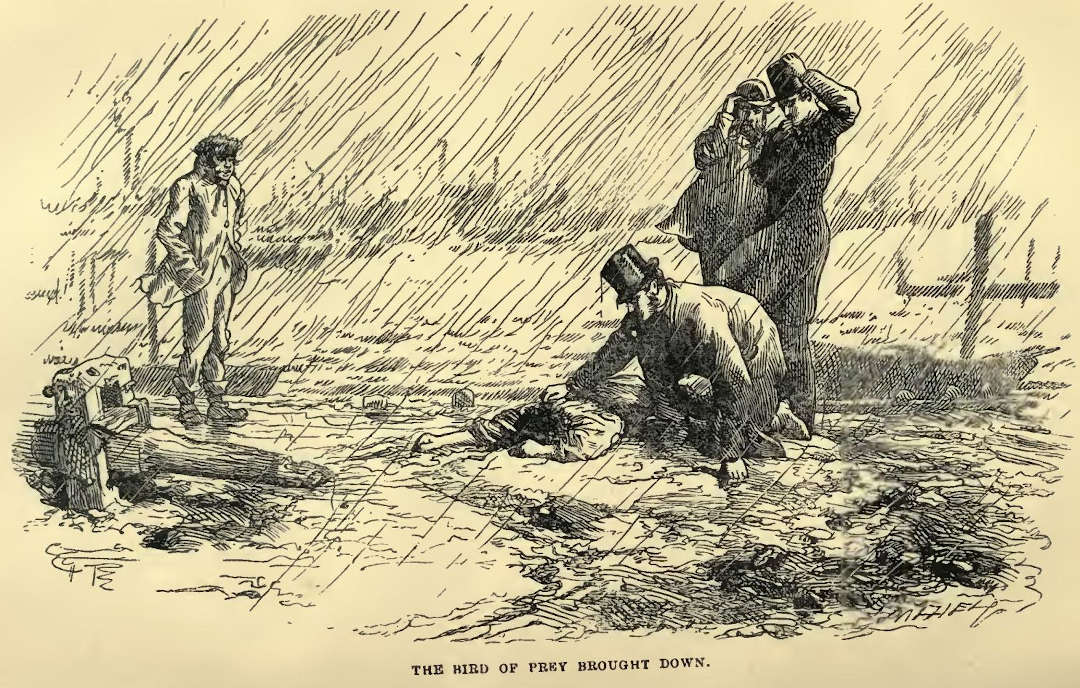
\includegraphics[scale=2.3]{01-14-01}

They ran to the rope, leaving him gasping there. Soon, the form of the
bird of prey, dead some hours, lay stretched upon the shore, with a new
blast storming at it and clotting the wet hair with hail-stones.

Father, was that you calling me? Father! I thought I heard you call me
twice before! Words never to be answered, those, upon the earth-side
of the grave. The wind sweeps jeeringly over Father, whips him with the
frayed ends of his dress and his jagged hair, tries to turn him where he
lies stark on his back, and force his face towards the rising sun, that
he may be shamed the more. A lull, and the wind is secret and prying
with him; lifts and lets falls a rag; hides palpitating under another
rag; runs nimbly through his hair and beard. Then, in a rush, it cruelly
taunts him. Father, was that you calling me? Was it you, the voiceless
and the dead? Was it you, thus buffeted as you lie here in a heap? Was
it you, thus baptized unto Death, with these flying impurities now flung
upon your face? Why not speak, Father? Soaking into this filthy ground
as you lie here, is your own shape. Did you never see such a shape
soaked into your boat? Speak, Father. Speak to us, the winds, the only
listeners left you!

‘Now see,’ said Mr Inspector, after mature deliberation: kneeling on one
knee beside the body, when they had stood looking down on the drowned
man, as he had many a time looked down on many another man: ‘the way of
it was this. Of course you gentlemen hardly failed to observe that he
was towing by the neck and arms.’

They had helped to release the rope, and of course not.

‘And you will have observed before, and you will observe now, that this
knot, which was drawn chock-tight round his neck by the strain of his
own arms, is a slip-knot’: holding it up for demonstration.

Plain enough.

‘Likewise you will have observed how he had run the other end of this
rope to his boat.’

It had the curves and indentations in it still, where it had been twined
and bound.

‘Now see,’ said Mr Inspector, ‘see how it works round upon him. It’s a
wild tempestuous evening when this man that was,’ stooping to wipe
some hailstones out of his hair with an end of his own drowned jacket,
‘--there! Now he’s more like himself; though he’s badly bruised,--when
this man that was, rows out upon the river on his usual lay. He carries
with him this coil of rope. He always carries with him this coil of
rope. It’s as well known to me as he was himself. Sometimes it lay in
the bottom of his boat. Sometimes he hung it loose round his neck.
He was a light-dresser was this man;--you see?’ lifting the loose
neckerchief over his breast, and taking the opportunity of wiping the
dead lips with it--‘and when it was wet, or freezing, or blew cold, he
would hang this coil of line round his neck. Last evening he does this.
Worse for him! He dodges about in his boat, does this man, till he gets
chilled. His hands,’ taking up one of them, which dropped like a leaden
weight, ‘get numbed. He sees some object that’s in his way of business,
floating. He makes ready to secure that object. He unwinds the end of
his coil that he wants to take some turns on in his boat, and he takes
turns enough on it to secure that it shan’t run out. He makes it too
secure, as it happens. He is a little longer about this than usual, his
hands being numbed. His object drifts up, before he is quite ready for
it. He catches at it, thinks he’ll make sure of the contents of the
pockets anyhow, in case he should be parted from it, bends right over
the stern, and in one of these heavy squalls, or in the cross-swell of
two steamers, or in not being quite prepared, or through all or most or
some, gets a lurch, overbalances and goes head-foremost overboard. Now
see! He can swim, can this man, and instantly he strikes out. But in
such striking-out he tangles his arms, pulls strong on the slip-knot,
and it runs home. The object he had expected to take in tow, floats by,
and his own boat tows him dead, to where we found him, all entangled
in his own line. You’ll ask me how I make out about the pockets? First,
I’ll tell you more; there was silver in ‘em. How do I make that out?
Simple and satisfactory. Because he’s got it here.’ The lecturer held up
the tightly clenched right hand.

‘What is to be done with the remains?’ asked Lightwood.

‘If you wouldn’t object to standing by him half a minute, sir,’ was
the reply, ‘I’ll find the nearest of our men to come and take charge of
him;--I still call it HIM, you see,’ said Mr Inspector, looking back as
he went, with a philosophical smile upon the force of habit.

‘Eugene,’ said Lightwood and was about to add ‘we may wait at a little
distance,’ when turning his head he found that no Eugene was there.

He raised his voice and called ‘Eugene! Holloa!’ But no Eugene replied.

It was broad daylight now, and he looked about. But no Eugene was in all
the view.

Mr Inspector speedily returning down the wooden stairs, with a police
constable, Lightwood asked him if he had seen his friend leave them? Mr
Inspector could not exactly say that he had seen him go, but had noticed
that he was restless.

‘Singular and entertaining combination, sir, your friend.’

‘I wish it had not been a part of his singular entertaining combination
to give me the slip under these dreary circumstances at this time of the
morning,’ said Lightwood. ‘Can we get anything hot to drink?’

We could, and we did. In a public-house kitchen with a large fire. We
got hot brandy and water, and it revived us wonderfully. Mr Inspector
having to Mr Riderhood announced his official intention of ‘keeping
his eye upon him’, stood him in a corner of the fireplace, like a wet
umbrella, and took no further outward and visible notice of that honest
man, except ordering a separate service of brandy and water for him:
apparently out of the public funds.

As Mortimer Lightwood sat before the blazing fire, conscious of drinking
brandy and water then and there in his sleep, and yet at one and the
same time drinking burnt sherry at the Six Jolly Fellowships, and
lying under the boat on the river shore, and sitting in the boat that
Riderhood rowed, and listening to the lecture recently concluded, and
having to dine in the Temple with an unknown man, who described himself
as M. H. F. Eugene Gaffer Harmon, and said he lived at Hailstorm,--as
he passed through these curious vicissitudes of fatigue and slumber,
arranged upon the scale of a dozen hours to the second, he became aware
of answering aloud a communication of pressing importance that had
never been made to him, and then turned it into a cough on beholding
Mr Inspector. For, he felt, with some natural indignation, that that
functionary might otherwise suspect him of having closed his eyes, or
wandered in his attention.

‘Here just before us, you see,’ said Mr Inspector.

‘I see,’ said Lightwood, with dignity.

‘And had hot brandy and water too, you see,’ said Mr Inspector, ‘and
then cut off at a great rate.’

‘Who?’ said Lightwood.

‘Your friend, you know.’

‘I know,’ he replied, again with dignity.

After hearing, in a mist through which Mr Inspector loomed vague and
large, that the officer took upon himself to prepare the dead man’s
daughter for what had befallen in the night, and generally that he took
everything upon himself, Mortimer Lightwood stumbled in his sleep to
a cab-stand, called a cab, and had entered the army and committed a
capital military offence and been tried by court martial and found
guilty and had arranged his affairs and been marched out to be shot,
before the door banged.

Hard work rowing the cab through the City to the Temple, for a cup of
from five to ten thousand pounds value, given by Mr Boffin; and hard
work holding forth at that immeasurable length to Eugene (when he had
been rescued with a rope from the running pavement) for making off in
that extraordinary manner! But he offered such ample apologies, and was
so very penitent, that when Lightwood got out of the cab, he gave
the driver a particular charge to be careful of him. Which the driver
(knowing there was no other fare left inside) stared at prodigiously.

In short, the night’s work had so exhausted and worn out this actor in
it, that he had become a mere somnambulist. He was too tired to rest in
his sleep, until he was even tired out of being too tired, and dropped
into oblivion. Late in the afternoon he awoke, and in some anxiety sent
round to Eugene’s lodging hard by, to inquire if he were up yet?

Oh yes, he was up. In fact, he had not been to bed. He had just come
home. And here he was, close following on the heels of the message.

‘Why what bloodshot, draggled, dishevelled spectacle is this!’ cried
Mortimer.

‘Are my feathers so very much rumpled?’ said Eugene, coolly going up to
the looking-glass. They ARE rather out of sorts. But consider. Such a
night for plumage!’

‘Such a night?’ repeated Mortimer. ‘What became of you in the morning?’

‘My dear fellow,’ said Eugene, sitting on his bed, ‘I felt that we
had bored one another so long, that an unbroken continuance of those
relations must inevitably terminate in our flying to opposite points of
the earth. I also felt that I had committed every crime in the Newgate
Calendar. So, for mingled considerations of friendship and felony, I
took a walk.’



